\model{Drawing and Tracing}

Open \textit{Drawing.java} and run the program.
Keep an eye on both the Drawing window and the Console output.
Notice the order in which the shapes are drawn.
Run the program again, as needed, so that all team members can see its behavior.
Then answer the questions below to explore and discuss the source code as a team.

\begin{multicols}{2}

\begin{center}
\textbf{Drawing (cropped)}
\end{center}

\fbox{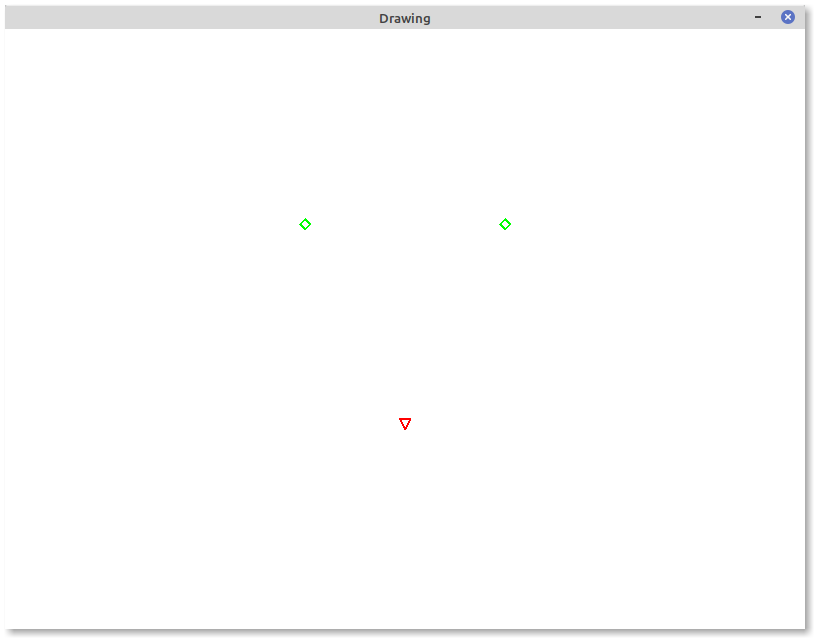
\includegraphics[trim=200 175 200 175,clip,width=\linewidth]{Drawing.png}}

\columnbreak

\begin{center}
\textbf{Console output}
\end{center}

\vspace{-1em}

\begin{javalst}
  diamond(300, 200)
      triangle(400, 400)
  diamond(500, 200)
\end{javalst}

\end{multicols}


\quest{15 min}


\Q Fill in each blank with IS-A, HAS-A, or USES-A:

\setlength{\defaultwidth}{5em}

\begin{multicols}{2}
\begin{enumerate}
\item Drawing \ans{IS-A}~   Canvas
\item Drawing \ans{HAS-A}~  Graphics2D
\item Drawing \ans{USES-A}~ Color
\item Drawing \ans{USES-A}~ JFrame
\end{enumerate}
\end{multicols}


\Q Based on the \java{Drawing()} constructor:

\begin{multicols}{2}
\begin{enumerate}
\item What is the Canvas width? \ans{800}
\item What is the Canvas height? \ans{600}
   \\
\item What is the JFrame title? \ans{\str{Drawing}}
\item What is ``in'' the JFrame? \ans{\jans{this}}
   \\ \textit{Hint:} see Line 33.
\end{enumerate}
\end{multicols}


\Q Summarize in your own words what each method does:

\begin{enumerate}

\item \java{paint(Graphics g)}

\begin{answer}[2em]
Called by the window toolkit to paint this Canvas.
Initializes \jans{this.g2} and calls the \jans{draw()} method.
Prevents the \jans{draw()} method from being called multiple times.
\end{answer}

\item \java{draw()}

\begin{answer}[2em]
Calls the \jans{diamond}, \jans{triangle}, and \jans{trace} methods to draw the shapes and debugging output.
Uses specific coordinates for each of the shapes.
\end{answer}

\end{enumerate}


\Q What is the purpose of the \java{g2} attribute? (i.e., How is it used in the program?)

\begin{answer}[3em]
The \jans{diamond} and \jans{triangle} methods use \java{g2} to do the actual drawing.
It provides methods like \java{setColor} and \java{drawLine}.
\end{answer}


\Q Consider the ``Console output'' (from \ref{\currfilename}) and the \java{trace()} method:

\begin{enumerate}

\item Why is the ``triangle'' line indented?

\begin{answer}[2em]
The \java{trace} method was called with \java{level} set to 1.
\end{answer}

\item Why are the ``diamond'' lines \emph{not} indented?

\begin{answer}[2em]
The \jans{level} was 0, and the loop (in \java{trace}) repeats \java{level} times.
\end{answer}

\item How long is the delay after drawing each shape?

\begin{answer}[2em]
500 milliseconds (i.e., 1/2 second).
\end{answer}

\end{enumerate}


\Q \label{key1}
Modify the \java{draw()} method to draw and trace many diamonds and triangles.
Use \java{for} loops to put each shape at a different $(x,y)$ location.
Reduce the \java{DELAY} so you can see the final result.
Paste your source code below:

\begin{answer}[15em]
Answers will vary; this one fills up most of the canvas:
\vspace{1em}
\begin{javaans}
for (int x = 20; x < 780; x += 20) {
    for (int y = 20; y < 580; y += 20) {
        diamond(x, y);
        trace(0, "diamond(%d, %d)", x, y);

        triangle(x + 10, y + 10);
        trace(1, "triangle(%d, %d)", x + 10, y + 10);
    }
}
\end{javaans}
\end{answer}
